%
% Erstellt von Daniel Falkner
% daniel.falkner@akad.de
% 
\documentclass[xcolor=dvipsnames]{beamer}
\usepackage[T1]{fontenc}
\usepackage[utf8]{inputenc}
\usepackage[ngerman]{isodate}
\usepackage[justification=centering,figurename=Abb.]{caption}
\usepackage{listings}
\usepackage{color}
\usepackage{dirtree}

\definecolor{mygreen}{rgb}{0,0.6,0}
\definecolor{mygray}{rgb}{0.5,0.5,0.5}
\definecolor{mymauve}{rgb}{0.58,0,0.82}

\lstdefinelanguage{JavaScript}{
  keywords={break, case, catch, continue, debugger, default, delete, do, else, finally, for, function, if, in, instanceof, new, return, switch, this, throw, try, typeof, var, void, while, with},
  morecomment=[l]{//},
  morecomment=[s]{/*}{*/},
  morestring=[b]',
  morestring=[b]",
  sensitive=true
}

\lstdefinelanguage{CSS}
{morekeywords={color,background,margin, font, width, float, height, padding, box, opacity, border, right, top, shadow, radius, bottom},
sensitive=false,
morecomment=[l]{//},
morecomment=[s]{/*}{*/},
morestring=[b]",
} 

\lstset{ %
  backgroundcolor=\color{white},   % choose the background color; you must add \usepackage{color} or \usepackage{xcolor}
  basicstyle=\footnotesize,        % the size of the fonts that are used for the code
  breakatwhitespace=false,         % sets if automatic breaks should only happen at whitespace
  breaklines=true,                 % sets automatic line breaking
  captionpos=b,                    % sets the caption-position to bottom
  commentstyle=\color{mygreen},    % comment style
  deletekeywords={...},            % if you want to delete keywords from the given language
  escapeinside={\%*}{*)},          % if you want to add LaTeX within your code
  extendedchars=true,              % lets you use non-ASCII characters; for 8-bits encodings only, does not work with UTF-8
 % frame=single,                    % adds a frame around the code
  keepspaces=true,                 % keeps spaces in text, useful for keeping indentation of code (possibly needs columns=flexible)
  keywordstyle=\color{blue},       % keyword style
  language=Octave,                 % the language of the code
  morekeywords={*,...},            % if you want to add more keywords to the set
  numbers=left,                    % where to put the line-numbers; possible values are (none, left, right)
  numbersep=5pt,                   % how far the line-numbers are from the code
  numberstyle=\tiny\color{mygray}, % the style that is used for the line-numbers
  rulecolor=\color{black},         % if not set, the frame-color may be changed on line-breaks within not-black text (e.g. comments (green here))
  showspaces=false,                % show spaces everywhere adding particular underscores; it overrides 'showstringspaces'
  showstringspaces=false,          % underline spaces within strings only
  showtabs=true,                  % show tabs within strings adding particular underscores
  stepnumber=1,                    % the step between two line-numbers. If it's 1, each line will be numbered
  stringstyle=\color{mymauve},     % string literal style
  tabsize=2,                       % sets default tabsize to 2 spaces
  title=\lstname,                   % show the filename of files included with \lstinputlisting; also try caption instead of title
  belowskip= 0pt 
}

\usetheme{Warsaw}
\usecolortheme[named=OliveGreen]{structure}
\renewcommand\thempfootnote{\arabic{mpfootnote}}

\newcommand*{\Title}{Präsentation der Umfragewebseite} %Titel
\subtitle{Modul DBA02} %Untertitel
\newcommand*{\Author}{Daniel Falkner + Eugen Grinschuk} %Name
\institute{AKAD Pinneberg + Stuttgart} %Uni
\titlegraphic{
\includegraphics[scale=0.2]{akad_logo.png}} %Logo

\title{\Title}
\author{\Author}
\date{3+4.Oktober.2013}

%Pdf Metainformationen
\subject{\Title}
\keywords{}

\begin{document}

%Titelseite
\begin{frame}
    \titlepage
\end{frame}

%Logo auf allen weiteren Folien
%\logo{
\includegraphics[scale=0.1]{akad_logo.png}}

%Inhaltsverzeichniss
\frame{\tableofcontents[hideothersubsections]} 


\section{Über uns}
\begin{frame} %%Eine Folie
  \frametitle{Über uns} %%Folientitel
  \begin{block}{Wer sind wir?}
	  \begin{itemize}
	  	\item AKAD Studenten - Bachelor of Science (Wirtschaftsinformatik)
	  \end{itemize}
  \end{block}
\end{frame}

\subsection{Daniel Falkner}
\begin{frame} %%Eine Folie
  \frametitle{Über uns} %%Folientitel
  \framesubtitle{Daniel Falkner} %%Fielenuntertitel
  \begin{block}{Daniel Falkner}
	  \begin{itemize}
  		\item T-Systems International GmbH - Telekom IT
  		\item IT-Architekt - System Analyst
		\item Projektleiter
		\item Proof of Concept Engineer
  		\item Debian Linux Administrator
	  \end{itemize}
  \end{block}
\end{frame}

\subsection{Eugen Grinschuk}
\begin{frame} %%Eine Folie
  \frametitle{Über uns} %%Folientitel
  \framesubtitle{Eugen Grinschuk} %%Fielenuntertitel
  \begin{block}{Eugen Grinschuk}
	  \begin{itemize}
  		\item T-Systems International GmbH
		\item IT-Architekt
  		\item Projektleiter
  		\item System Engineer
	  \end{itemize}
  \end{block}
\end{frame}


\section{Werkzeuge}
\begin{frame} %%Eine Folie
  \frametitle{verwendete Werkzeuge} %%Folientitel
  \begin{block}{}
	  \begin{itemize}
  		\item > PHP 5.3
		\item MySQL 5
  		\item Eclipse
  		\item Git
  		\item Dia \footnote{\url{http://live.gnome.org/Dia}}
  		\item \url{http://www.dba02.studieren-und-arbeiten.de}
	  \end{itemize}
  \end{block}  
\end{frame}


\section{Datenbank}
\begin{frame} %%Eine Folie
  \frametitle{Datenbank} %%Folientitel
  \tableofcontents[currentsection, hideothersubsections]
\end{frame}


\subsection{UML Modell}
\begin{frame} %%Eine Folie
  \frametitle{UML Modell} %%Folientitel
  	\begin{figure}
	   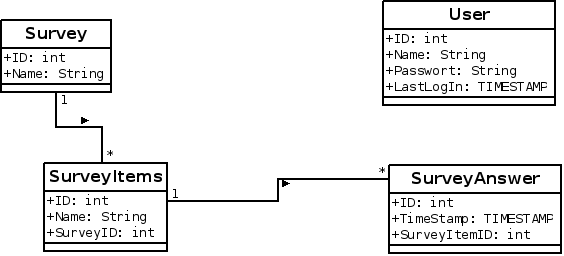
\includegraphics[scale=0.4]{database.png}
		\caption{UML Modell}
	\end{figure}
	\begin{block}{}		
	\begin{itemize}[]
		\item Flache Struktur
		\item Minimaler Aufbau für Umfragesystem mit Usern
	\end{itemize}
\end{block}\end{frame}

\subsection{Relationen Modell}
\begin{frame} %%Eine Folie

	\begin{block}{Relationen Modell}		
		\begin{itemize}[]
			\item 3te Normalform
			\item Keine Redundanz
		\end{itemize}
	\end{block}


\begin{table}
\begin{tabular}{|l|l|} \hline\hline
\textbf{ID} & \textbf{Name} \\
\hline
1 & Wie findest du dieses Seite? \\
\hline\hline
\end{tabular}
\caption{Survey}
\end{table}

\end{frame}


\begin{frame} %%Eine Folie
  \frametitle{Relationen Modell} %%Folientitel
\begin{table}
\begin{tabular}{|l|l|l|} \hline\hline
\textbf{ID} & \textbf{Name} & \textbf{SurveyID}\\
\hline
1 & Super & 1 \\
2 & Fett & 1 \\
\hline\hline
\end{tabular}
\caption{SurveyItems}
\end{table}



\begin{table}
\begin{tabular}{|l|l|r|} \hline\hline
\textbf{ID} & \textbf{TimeStamp}  & \textbf{SurveyItemID}\\
\hline
1 & 2013-08-29 19:53:55 & 2 \\
2 & 2013-08-29 19:53:55 & 1 \\
\hline\hline
\end{tabular}
\caption{SurveyAnswer}
\end{table}

\end{frame}


\begin{frame} %%Eine Folie
  \frametitle{Relationen Modell} %%Folientitel

\begin{table}
\begin{tabular}{|l|l|l|l|} \hline\hline
\textbf{ID} & \textbf{Name}  & \textbf{Passwort} & \textbf{LastLogIn}\\
\hline
1 & admin & test & 0000-00-00 00:00:00 \\
\hline\hline
\end{tabular}
  \caption{User}
  \end{table}

	\begin{block}{}		
		\begin{itemize}[]
			\item Gute Performance 
		\end{itemize}
	\end{block}

\end{frame}


\subsection{SQL DDL}
\begin{frame}[fragile] %%Eine Folie
\frametitle{SQL Data Definition Language} %%Folientitel

\begin{lstlisting}[language=SQL, caption=database.sql]
CREATE TABLE `Survey` (
 `ID` int(11) NOT NULL AUTO_INCREMENT,
 `Name` varchar(255) NOT NULL,
 PRIMARY KEY (`ID`)
) ENGINE=InnoDB AUTO_INCREMENT=0 DEFAULT CHARSET=latin1;
\end{lstlisting} 
\end{frame}

\begin{frame}[fragile] %%Eine Folie
\frametitle{SQL Data Definition Language} %%Folientitel

\begin{lstlisting}[language=SQL, caption=database.sql]
CREATE TABLE `SurveyItems` (
 `ID` int(11) NOT NULL AUTO_INCREMENT,
 `Name` varchar(255) NOT NULL,
 `SurveyID` int(11) NOT NULL,
 PRIMARY KEY (`ID`),
 KEY `SurveyID` (`SurveyID`),
 CONSTRAINT `SurveyItems_ibfk_2` FOREIGN KEY (`SurveyID`) REFERENCES `Survey` (`ID`) ON DELETE CASCADE ON UPDATE CASCADE
) ENGINE=InnoDB AUTO_INCREMENT=0 DEFAULT CHARSET=latin1;
\end{lstlisting} 
\end{frame}

\begin{frame}[fragile] %%Eine Folie
\frametitle{SQL Data Definition Language} %%Folientitel
\begin{lstlisting}[language=SQL, caption=database.sql]
CREATE TABLE `SurveyAnswer` (
 `ID` int(11) NOT NULL AUTO_INCREMENT,
 `TimeStamp` timestamp NOT NULL DEFAULT CURRENT_TIMESTAMP,
 `SurveyItemID` int(11) NOT NULL,
 PRIMARY KEY (`ID`),
 KEY `SurveyItemID` (`SurveyItemID`),
 CONSTRAINT `SurveyAnswer_ibfk_2` FOREIGN KEY (`SurveyItemID`) REFERENCES `SurveyItems` (`ID`) ON DELETE CASCADE ON UPDATE CASCADE
) ENGINE=InnoDB AUTO_INCREMENT=0 DEFAULT CHARSET=latin1;
\end{lstlisting} 
\end{frame}


\begin{frame}[fragile] %%Eine Folie
\frametitle{SQL Data Definition Language} %%Folientitel
\begin{lstlisting}[language=SQL, caption=database.sql]
CREATE TABLE `User` (
 `ID` int(11) NOT NULL AUTO_INCREMENT,
 `Name` varchar(64) NOT NULL,
 `Passwort` varchar(64) NOT NULL,
 `LastLogIn` timestamp NOT NULL DEFAULT '0000-00-00 00:00:00',
 PRIMARY KEY (`ID`),
 UNIQUE KEY `Name` (`Name`)
) ENGINE=InnoDB AUTO_INCREMENT=0 DEFAULT CHARSET=latin1;
\end{lstlisting} 
\end{frame}

\begin{frame}[fragile] %%Eine Folie
\frametitle{SQL Data Definition Language} %%Folientitel
\begin{lstlisting}[language=SQL, caption=database.sql]
INSERT INTO `User` (
 `ID` ,
 `Name` ,
 `Passwort` ,
 `LastLogIn`
) VALUES (
 NULL , 'admin', 'test', '0000-00-00 00:00:00'
);
\end{lstlisting} 
\end{frame}


\section{Programmcode}
\begin{frame}[shrink] %%Eine Folie
  \frametitle{Programmcode} %%Folientitel
  \tableofcontents[currentsection, hideothersubsections]

\end{frame}

\subsection{PHP}
\begin{frame} %%Eine Folie
  \frametitle{> PHP 5.3} %%Folientitel
  \begin{block}{}
	  \begin{itemize}
  		\item OOP \footnote{Objektorientierte Programmierung}
		\item Namespaces
  		\item Klassen Autoloader
		\item 1426 Zeilen
		\begin{itemize}
			\item 525 Zeilen Code
			\item 526 Zeilen Kommentare
			\item 375 Leerzeilen ;-)
	        \end{itemize}
	  \end{itemize}
  \end{block} 
\end{frame}

\subsection{Design Pattern}
\begin{frame} %%Eine Folie
  \frametitle{Design Pattern} %%Folientitel
  \begin{block}{}
	  \begin{itemize}
  		\item Singleton für Konfiguration
  		\item MVC \footnote{Modell View Controller}
	  \end{itemize}
  \end{block} 
\end{frame}

\begin{frame}[fragile] %%Eine Folie
\frametitle{Singleton und Konfigruation in INI Datei} %%Folientitel

\begin{lstlisting}[language=PHP, caption=config.ini]
database_type = mysql
database_port = 3306
database_name = dba02
database_host = localhost
database_user = dbuser
database_pass = supersicherundextremgeheim
database_verbose = 0
application_debugging = 0
\end{lstlisting} 

\begin{lstlisting}[language=PHP, caption=Config Klasse]
$conf = \Config::getInstance();
$debug = $conf->application_debugging;
\end{lstlisting} 

\end{frame}


\begin{frame} %%Eine Folie
\frametitle{MVC} %%Folientitel
\begin{figure}
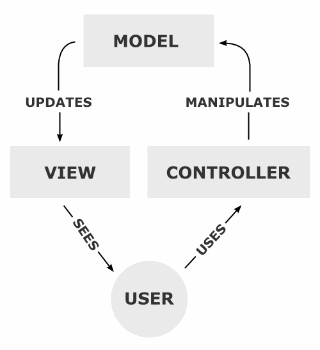
\includegraphics[scale=0.4]{MVC-Process.png}
\caption{Wikipedia MVC \\ \tiny{\textcolor{gray}{\url{http://en.wikipedia.org/wiki/File:MVC-Process.png}}}}
\end{figure}
\end{frame}


\subsection{Controller}
\begin{frame} %%Eine Folie
  \frametitle{Die Steuerung} %%Folientitel
  \begin{block}{}
	  \begin{itemize}
  		\item Interface zwischen Model und View
  		\item Saubere Codekapselung
  		\item kein Spagetti Code und Springen zwischen Dateien
	  \end{itemize}
  \end{block} 
\end{frame}

\subsection{View}
\begin{frame}[fragile] %%Eine Folie
  \frametitle{Präsentation} %%Folientitel
  \begin{block}{}
	  \begin{itemize}
  		\item eigene Template Engine
  		\item CSS Twitter Bootstrap \footnote{\url{http://getbootstrap.com/}}
	  \end{itemize}
  \end{block}
  
\begin{lstlisting}[language=PHP, caption=Template Engine]
$this->view->setTemplate('surveys');
$this->view->assign('surveys', $this->model->getSurveys());
$this->view->display();
\end{lstlisting} 

\end{frame}

\subsection{Model}
\begin{frame} %%Eine Folie
  \frametitle{Modell} %%Folientitel
  \begin{block}{}
	  \begin{itemize}
  		\item PDO \footnote{PHP Data Objects}
  		\item Prepared Statements
  		\item SQL-Injection Vorbeugung
	  \end{itemize}
  \end{block} 
\end{frame}

\begin{frame}[fragile] %%Eine Folie
  \frametitle{SQL-Injection Beispiel} %%Folientitel

\begin{lstlisting}[language=PHP, caption=PHP Code der nicht Existieren sollte!!]
$user = $_GET['user'];
$sql = "SELECT * FROM user WHERE name = '$user'";
\end{lstlisting} 

\begin{block}{URL Aufruf}
http://meineseite.de/index.php?user=owned'; DROP TABLE user;
\end{block}
 
  \begin{alertblock}{Das Ausgeführte SQL Query}
SELECT * FROM table WHERE key = 'owned'; DROP TABLE user;
	\end{alertblock} 


\end{frame}

\section{Live Demo}
\begin{frame} %%Eine Folie
  \frametitle{Live Demo} %%Folientitel
  \begin{center}  
      \Huge	Please wait ... we are connecting ;-)
  \end{center}
\end{frame}


\section{Anhang}
\begin{frame}
  \frametitle{Anhang} %%Folientitel
	\begin{block}{}	
		\begin{center}
			Vielen Dank für Ihre Aufmerksamkeit. \\
			Fragen?
		\end{center}	
	\end{block}
	\begin{block}{Links}	
		\begin{itemize}
			\item \url{https://github.com/derdanu/akad-dba02-beamer}	
			\item \url{http://www.dba02.studieren-und-arbeiten.de}					
		\end{itemize}
	\end{block}
\end{frame}

\subsection{Quellen}
\begin{frame} %%Eine Folie
  \frametitle{Quellen} %%Folientitel
 	\begin{itemize}
		\item \url{http://www.w3.org/}
		\item \url{http://git-scm.com/}
		\item \url{http://de.selfhtml.org/}
		\item \url{http://php.net/}
		\item \url{http://openbook.galileocomputing.de/javascript_ajax/}
	\end{itemize}
\end{frame}




\end{document}


